% =============================================================================
% CAPÍTULO 1 — a raiz: o número e a barra.
%
% O fracasso que o abre, com número na mão: os últimos \numFracaoCurtaDias{} pregões do índice
% tiveram \numFracaoCurtaPct\% de dias de alta e os últimos \numFracaoLongaDias{} tiveram
% \numFracaoLongaPct\% — dois números para a mesma pergunta, e nada na aritmética diz se a
% diferença é do mundo ou do tamanho da janela. A barra diz: os \numFracaoDiferencaPct{} pontos
% são \numFracaoDiferencaBarras{} barras da janela curta.
%
% Medição: lab/experimentos/E21_proporcao.ipynb. Figuras: figuras/E21_proporcao_*.
% =============================================================================

\chapter{O número e a barra}
\label{cap:barra}

\section{Dois números para a mesma pergunta}

Um índice fecha o dia, e a pergunta mais simples que se faz sobre ele cabe numa linha: o que
costuma acontecer aqui? Quem responde é a média. Some os dias e divida pelo número deles, e o
resultado é a resposta que todo mundo aceita sem pedir mais nada.

Vale fazer a conta com o dado na mão, num índice de \numBarraSerieDias{} pregões. Nos últimos
\numFracaoCurtaDias{} deles, o índice subiu em \numFracaoCurtaPct\% dos dias. Nos últimos
\numFracaoLongaDias{}, subiu em \numFracaoLongaPct\%. A mesma série, a mesma conta e a mesma
pergunta, com \numFracaoDiferencaPct{} pontos de diferença entre as duas respostas.

Uma das duas mentiu, ou as duas valem e a pergunta não estava bem feita. O que se pode dizer
sem mais nada é pouco: uma janela é doze vezes mais longa que a outra, e nada na aritmética
avisa se a diferença veio do mundo que mudou ou do tamanho do pedaço que se olhou. É essa
segunda possibilidade que a medição precisa separar, porque ela existe sempre, mesmo num mundo
parado, e sem medi-la não há como ler a primeira.

\section{O sorteio, a lei e a variável}

Três palavras, e cada uma entra porque a conta acima precisou dela.

% aterramento: sorteio
Um \textbf{sorteio} é o ato de tirar um resultado de um conjunto de resultados possíveis. A
% aterramento: lei
\textbf{lei} é o que diz a chance de cada um: uma moeda honesta dá cara em metade dos sorteios,
% aterramento: probabilidade
e um dado viciado dá seis em metade deles.
A \textbf{probabilidade} de um resultado é a fração
de vezes que ele sai quando o sorteio se repete muitas vezes --- com muitos sorteios, a fração
se aquieta em torno de um número, e é esse número que se chama de probabilidade.

Vale ver a aquietação com números pequenos. Numa moeda honesta, quatro sorteios dão duas caras
por sorte, mas dão uma, três e até zero com frequência; quatro mil sorteios dão perto de duas
mil caras, e a distância entre a fração obtida e a metade encolhe à medida que o número de
sorteios cresce. A medição usa esse encolhimento como régua.

% aterramento: variavel-aleatoria
% aterramento: X
% aterramento: p
O dia do índice é um sorteio, e a pergunta é sobre um resultado de dois valores: o
dia subiu ou o dia não subiu. Ao resultado do dia dá-se um número, e o número é a
\textbf{variável aleatória}: vale um quando o índice sobe e zero quando não sobe. A
média de uma lista desses números é a fração de dias de alta --- a conta das duas janelas, agora
com nome.

\section{A média de muitos sorteios}

% aterramento: dispersao
Falta a peça que responde à pergunta da abertura, e ela é a dispersão. A média de uma lista de
dias diz onde a lista fica; a \textbf{dispersão} diz de quanto essa média se mexeria se os dias
sorteados fossem outros. As duas andam juntas, e é a segunda que as duas janelas do índice
disputam.

% aterramento: esperanca
% aterramento: media-simbolo
% aterramento: media
Chame de $\E[X]$ a média da variável aleatória $X$ sobre muitos sorteios --- o número em torno
% aterramento: variancia
do qual os resultados se aquietam.
% aterramento: desvio
Chame de \textbf{variância} a média do quadrado do
afastamento dessa média, e de \textbf{desvio} a sua raiz: o desvio é o tamanho típico do
afastamento, na unidade do dado. Para a variável do dia, que vale um com probabilidade $p$ e
zero no resto, a média é $p$ e a variância é $p(1-p)$: o afastamento é $1-p$ quando o dia sobe
e $p$ quando não sobe, e a média dos quadrados dá $p(1-p)^2 + (1-p)p^2 = p(1-p)$.

Agora a pergunta da abertura tem forma. A fração de altas de uma janela de $n$ dias é a média
de $n$ sorteios, e o que se quer saber é de quanto ela se mexe por conta própria.

\begin{proposicao}[a barra da fração]\label{prop:barra}
% aterramento: barra
% aterramento: N
% aterramento: n
% aterramento: independencia
Se os $n$ dias de uma janela são sorteios independentes da mesma lei, com a mesma probabilidade
$p$ de alta, então a fração de altas tem média $p$ e desvio
$\sqrt{p(1-p)/n}$.
\end{proposicao}

\begin{proof}
Seja $N$ o número de altas na janela: $N$ é a soma dos $n$ valores do dia, cada um valendo um
com probabilidade $p$. A média de uma soma é a soma das médias, de modo que a média de $N$ é
$np$, e a média da fração $N/n$ é $p$.

Para o desvio, escreva $N^2 = N(N-1) + N$ e tome as médias. A média de $N$ é $np$. A média de
$N(N-1)$ conta os pares de dias distintos em que os dois subiram: são $n(n-1)$ pares, cada um
com probabilidade $p^2$ de subir nos dois dias, de modo que ela vale $n(n-1)p^2$. Então a média
de $N^2$ é $n(n-1)p^2 + np$, e a variância de $N$ é
\[
  n(n-1)p^2 + np - (np)^2 = np(1-p).
\]
Dividir $N$ por $n$ divide a variância por $n^2$ e o desvio por $n$, e é daí que sai
$\sqrt{p(1-p)/n}$.
\end{proof}

A independência é a hipótese que faz o trabalho: ela é o que permite multiplicar $p$ por $p$ no
par de dias, e é exatamente o que um mundo que muda viola. A proposição também diz o preço do
tamanho: o desvio cai com a raiz do número de dias, de modo que uma janela quatro vezes mais
longa tem a metade do desvio, e não um quarto.

Com $n = \numFracaoCurtaDias$ e $p = \numFracaoLongaPct\%$, a barra vale
\numBarraCurtaPct{} pontos; com $n = \numFracaoLongaDias$, \numBarraLongaPct{} pontos. A
diferença entre as duas janelas do índice --- \numFracaoDiferencaPct{} pontos --- é de
\numFracaoDiferencaBarras{} barras da janela curta. Ela cabe dentro da própria margem de erro,
e o que parecia o mundo mudando é a janela sendo curta.

\section{A barra que se confere}

Uma previsão que não se confere é uma opinião com símbolo. A barra se confere do jeito mais
direto que existe: sorteando mundos. Sorteiam-se \numMundos{} janelas de cada tamanho, todas
com a mesma probabilidade de alta, e mede-se a dispersão das frações obtidas contra a previsão
da \cref{prop:barra}.

\begin{table}[htbp]
  \centering
  \begin{tabular}{rrrr}
    \hline
    dias na & a barra & a dispersão & a razão \\
    janela & prevista (\%) & medida (\%) & medida/prevista \\
    \hline
    \numMundoVinteUmDias & \numMundoVinteUmPrevistoPct & \numMundoVinteUmMedidoPct & \numMundoVinteUmRazao \\
    \numMundoSessentaETresDias & \numMundoSessentaETresPrevistoPct & \numMundoSessentaETresMedidoPct & \numMundoSessentaETresRazao \\
    \numMundoDuzentosECinquentaEDoisDias & \numMundoDuzentosECinquentaEDoisPrevistoPct & \numMundoDuzentosECinquentaEDoisMedidoPct & \numMundoDuzentosECinquentaEDoisRazao \\
    \numMundoMilDuzentosESessentaDias & \numMundoMilDuzentosESessentaPrevistoPct & \numMundoMilDuzentosESessentaMedidoPct & \numMundoMilDuzentosESessentaRazao \\
    \hline
  \end{tabular}
  \caption{A barra prevista pela \cref{prop:barra} e a dispersão medida em \numMundos{}
    mundos sorteados, para quatro tamanhos de janela. A última coluna é a razão entre as duas,
    e ela fica perto de um em todas as linhas.}
  \label{tab:barra}
\end{table}

As quatro razões ficam entre \numMundoVinteUmRazao\ e \numMundoMilDuzentosESessentaRazao, com
o espalhamento que \numMundos{} sorteios admitem. A previsão não é um enfeite: ela acerta a
dispersão medida, e a \cref{fig:barra} mostra por quê --- no papel logarítmico as duas curvas
viram retas paralelas, e a inclinação delas é a da raiz.

\begin{figure}[htbp]
  \centering
  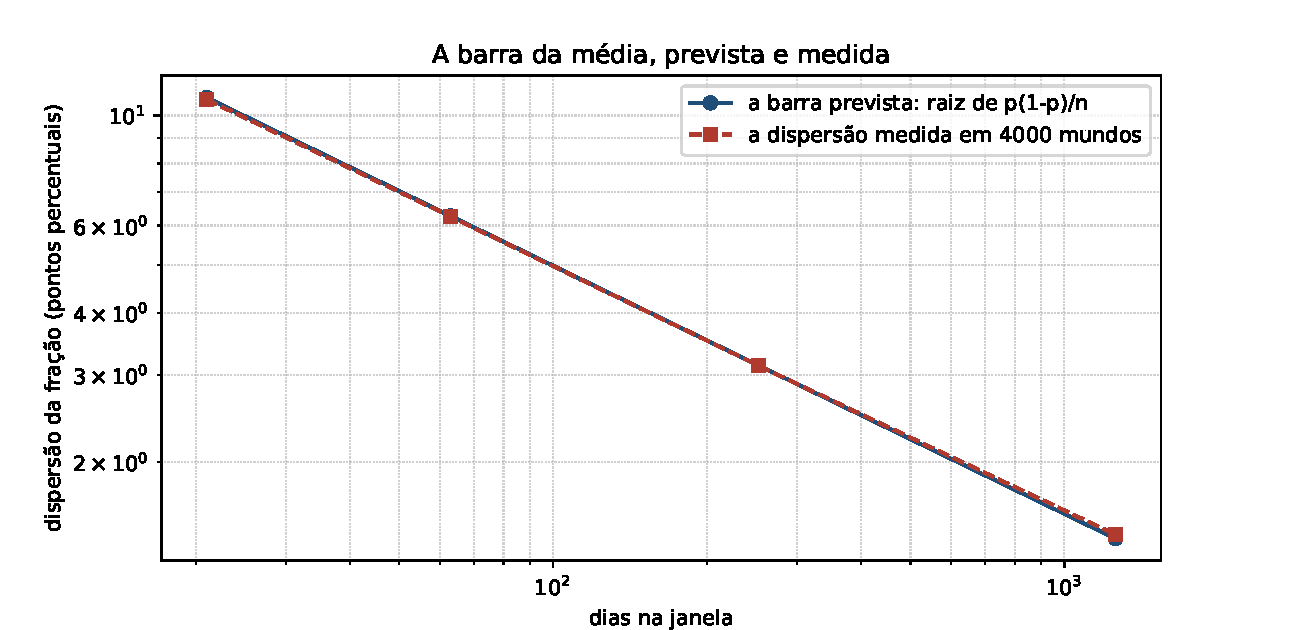
\includegraphics[width=\linewidth]{figuras/E21_proporcao_1.pdf}
  \caption{A barra da fração, prevista e medida, contra o número de dias na janela. Os dois
    eixos estão em escala logarítmica, de modo que uma queda pela raiz aparece como reta de
    inclinação menos um meio; as duas curvas caem juntas.}
  \label{fig:barra}
\end{figure}

\section{A barra no dado, e o que ela deixa de fora}

Falta a medição que interessa, e ela não precisa de mundo sorteado: a própria série tem
\numJanelasCurtasConta{} janelas de \numFracaoCurtaDias{} dias, uma para cada dia em que há
passado suficiente. Medir a fração de altas em cada uma delas dá a dispersão que o índice de
fato teve, sem escolher janela nenhuma.

A dispersão entre as \numJanelasCurtasConta{} janelas é de \numJanelasCurtasDispersaoPct{}
pontos, contra a barra de \numBarraCurtaPct{} pontos prevista para uma janela desse tamanho ---
uma razão de \numJanelasCurtasRazao. O dado real se comporta como sorteios independentes da
mesma lei, e essa é a leitura mais forte que a medição entrega: \textbf{o que muda no mercado não
é a média}. A fração de dias de alta atravessa vinte e seis anos sem se mexer mais do que o
próprio barulho dela.

\begin{figure}[htbp]
  \centering
  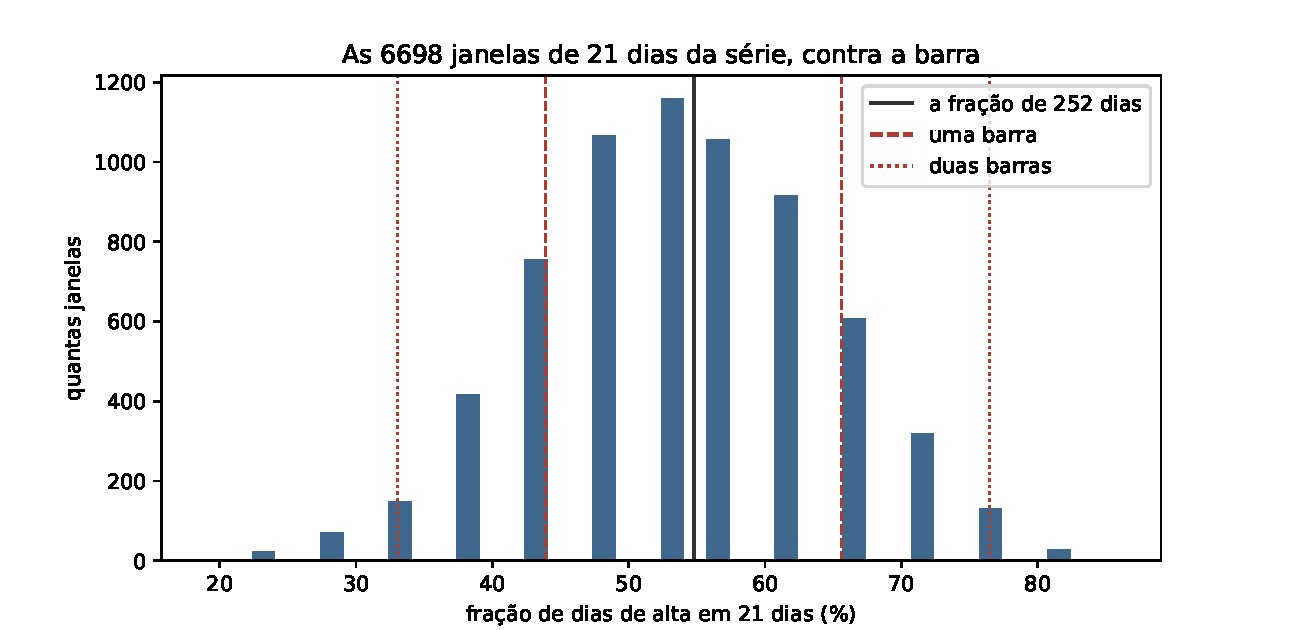
\includegraphics[width=\linewidth]{figuras/E21_proporcao_2.pdf}
  \caption{As \numJanelasCurtasConta{} janelas de \numFracaoCurtaDias{} dias da série. A linha
    cheia é a fração dos \numFracaoLongaDias{} dias; a tracejada fica a uma barra dela e a
    pontilhada a duas. A forma tem o corpo dentro de duas barras, com as pontas em
    \numJanelasCurtasMinimaPct\% e \numJanelasCurtasMaximaPct\%.}
  \label{fig:janelas}
\end{figure}

A forma da \cref{fig:janelas} confirma e limita ao mesmo tempo. Do lado de dentro, o corpo das
janelas cabe entre as duas barras, e só \numJanelasCurtasForaPct\% das janelas ficam fora ---
poucas, e por isso mesmo as pontas chamam atenção. Do lado de fora, as duas mais extremas
existem: uma janela com \numJanelasCurtasMinimaPct\% de altas e outra com
\numJanelasCurtasMaximaPct\%. Uma média de vinte e um dias não distingue um mundo calmo de um
mundo em que quase todo dia sobe, e é essa distância que a barra não cobre sozinha.

\section{O que fica}

Fica o instrumento mais antigo do livro, agora com o preço escrito: a média de $n$ sorteios
carrega o desvio $\sqrt{p(1-p)/n}$, medido em \numMundos{} mundos sorteados e conferido contra
o dado. E fica a leitura que as duas janelas da abertura não podiam dar sozinhas: os
\numFracaoDiferencaPct{} pontos de diferença entre elas valem
\numFracaoDiferencaBarras{} barras, e um número que cabe dentro da própria barra não é notícia.

A pergunta da noite, porém, não é sobre a média. Quem carrega uma posição não pergunta quanto o
índice sobe num dia comum; pergunta o tamanho do dia ruim, e a média não tem essa resposta: ela
é a mesma numa série calma e numa série que dá um salto por mês. Medir o dia ruim exige erguer
uma linha sobre os piores dias do passado e olhar o que ficou abaixo dela --- e é essa linha que
o capítulo seguinte constrói.
